\documentclass[12pt,a4paper]{article}
\usepackage[a4paper,margin=1in]{geometry}
\setlength{\headheight}{15pt}
\usepackage{graphicx}
\usepackage{booktabs}
\usepackage{amsmath,amssymb}
\usepackage{float}
\usepackage{hyperref}
\usepackage{xcolor}
\usepackage{listings}
\usepackage{enumitem}
\usepackage{fancyhdr}
\usepackage{longtable}

\hypersetup{colorlinks=true,linkcolor=blue,urlcolor=blue}

\pagestyle{fancy}
\fancyhf{}
\lhead{ICS1512}
\rhead{Machine Learning Algorithms Laboratory}
\cfoot{\thepage}

\lstset{
language=Python,
basicstyle=\ttfamily\footnotesize,
numbers=left,
numberstyle=\tiny\color{gray},
frame=single,
breaklines=true,
showstringspaces=false,
keywordstyle=\color{blue},
commentstyle=\color{gray},
stringstyle=\color{red}
}

\begin{document}

\begin{tabular}{|p{4cm}|p{11cm}|}
\hline
Experiment No. & 6\\ \hline
Experiment Title & Bagging, Boosting, and Stacked Ensemble Models\\ \hline
GitHub Repository & \href{https://github.com/rishirithesh/ML_Lab}{Click Here} \\ \hline
Jupyter Notebook & \href{https://github.com/rishirithesh/ML_Lab/blob/main/Assignment%206/Experiment_6_Ensemble_Learning.ipynb}{Click Here to View ML\_Lab\_Exp6.ipynb} \\ \hline
Student Name & Rishi Rithesh\\ \hline
Register Number & 3122247001049\\ \hline
Faculty & Dr. Poreddy Ajay Kumar Reddy \\ \hline
Submission Date & 21/09/2026\\ \hline
\end{tabular}

\vspace{0.4cm}

\section{Objective}
To understand the theoretical foundations, implementation mechanics, and comparative performance of the primary ensemble learning paradigms:
\begin{enumerate}[leftmargin=*]
    \item \textbf{Bagging (Bootstrap Aggregation):} Implementing parallel ensembles using Decision Tree base estimators to analyze variance reduction.
    \item \textbf{Boosting (Adaptive \& Gradient Boosting):} Implementing sequential boosting algorithms (\texttt{AdaBoostClassifier} and \texttt{GradientBoostingClassifier}) with systematically tuned learning rates and estimator depths to minimize residual bias.
    \item \textbf{Stacking (Stacked Generalization):} Constructing a heterogeneous multi-level ensemble combining Support Vector Machines (SVM), Gaussian Na\"ive Bayes, and Decision Trees via a Logistic Regression meta-learner.
    \item \textbf{Benchmarking \& Bias-Variance Analysis:} Benchmarking ensemble models against individual base classifiers using 5-fold Stratified Cross-Validation, ROC/PR curves, confusion matrices, and empirical bias-variance decomposition.
\end{enumerate}

\section{Problem Statement}
\textbf{Problem:} To classify breast tumors as either \textit{Malignant} or \textit{Benign} using nuclear cytological attributes, and evaluate how Bagging, Boosting, and Stacking improve predictive reliability, generalization capacity, and stability compared to single baseline learners.

\textbf{Input:} Wisconsin Diagnostic Breast Cancer (WDBC) dataset comprising 569 clinical biopsy records characterized by 30 continuous morphometric features describing nuclear size, shape, texture, and boundary irregularities.

\textbf{Output:} Cleaned and standardized feature matrices, Exploratory Data Analysis (EDA) visualizations, hyperparameter optimization tables (Tables 1, 2, and 3), comprehensive benchmark table (Table 4), multi-model confusion matrices, ROC/PR curves, feature importances, empirical bias-variance decomposition plots, and detailed analytical answers to observation questions.

\section{Dataset Description}
\begin{longtable}{|p{6cm}|p{8cm}|}
\hline
Dataset Name & Wisconsin Diagnostic Breast Cancer (WDBC) Dataset\\ \hline
Dataset Source & UCI Machine Learning Repository / \texttt{sklearn.datasets}\\ \hline
Number of Samples ($N$) & 569 patient biopsy cases\\ \hline
Number of Features ($p$) & 30 continuous cytological descriptors\\ \hline
Target Variable & \texttt{diagnosis} (Binary: Malignant / Benign)\\ \hline
Target Classes & 2 (Malignant: 212 [37.26\%], Benign: 357 [62.74\%])\\ \hline
Missing Values & 0 missing records across all features\\ \hline
Train-Test Partitioning & 80\% training (455 samples), 20\% testing (114 samples)\\ \hline
Validation Strategy & 5-Fold Stratified Cross-Validation\\ \hline
\end{longtable}

\section{Exploratory Data Analysis}
\begin{itemize}
    \item Class distribution analysis of biopsy outcomes
    \item Cytological feature distributions and kernel density estimations
    \item Pairwise correlation matrix and collinearity analysis
    \item Outlier boxplots and feature separability analysis
\end{itemize}

\subsection*{Figure: Class Distribution}
\begin{figure}[H]
\centering
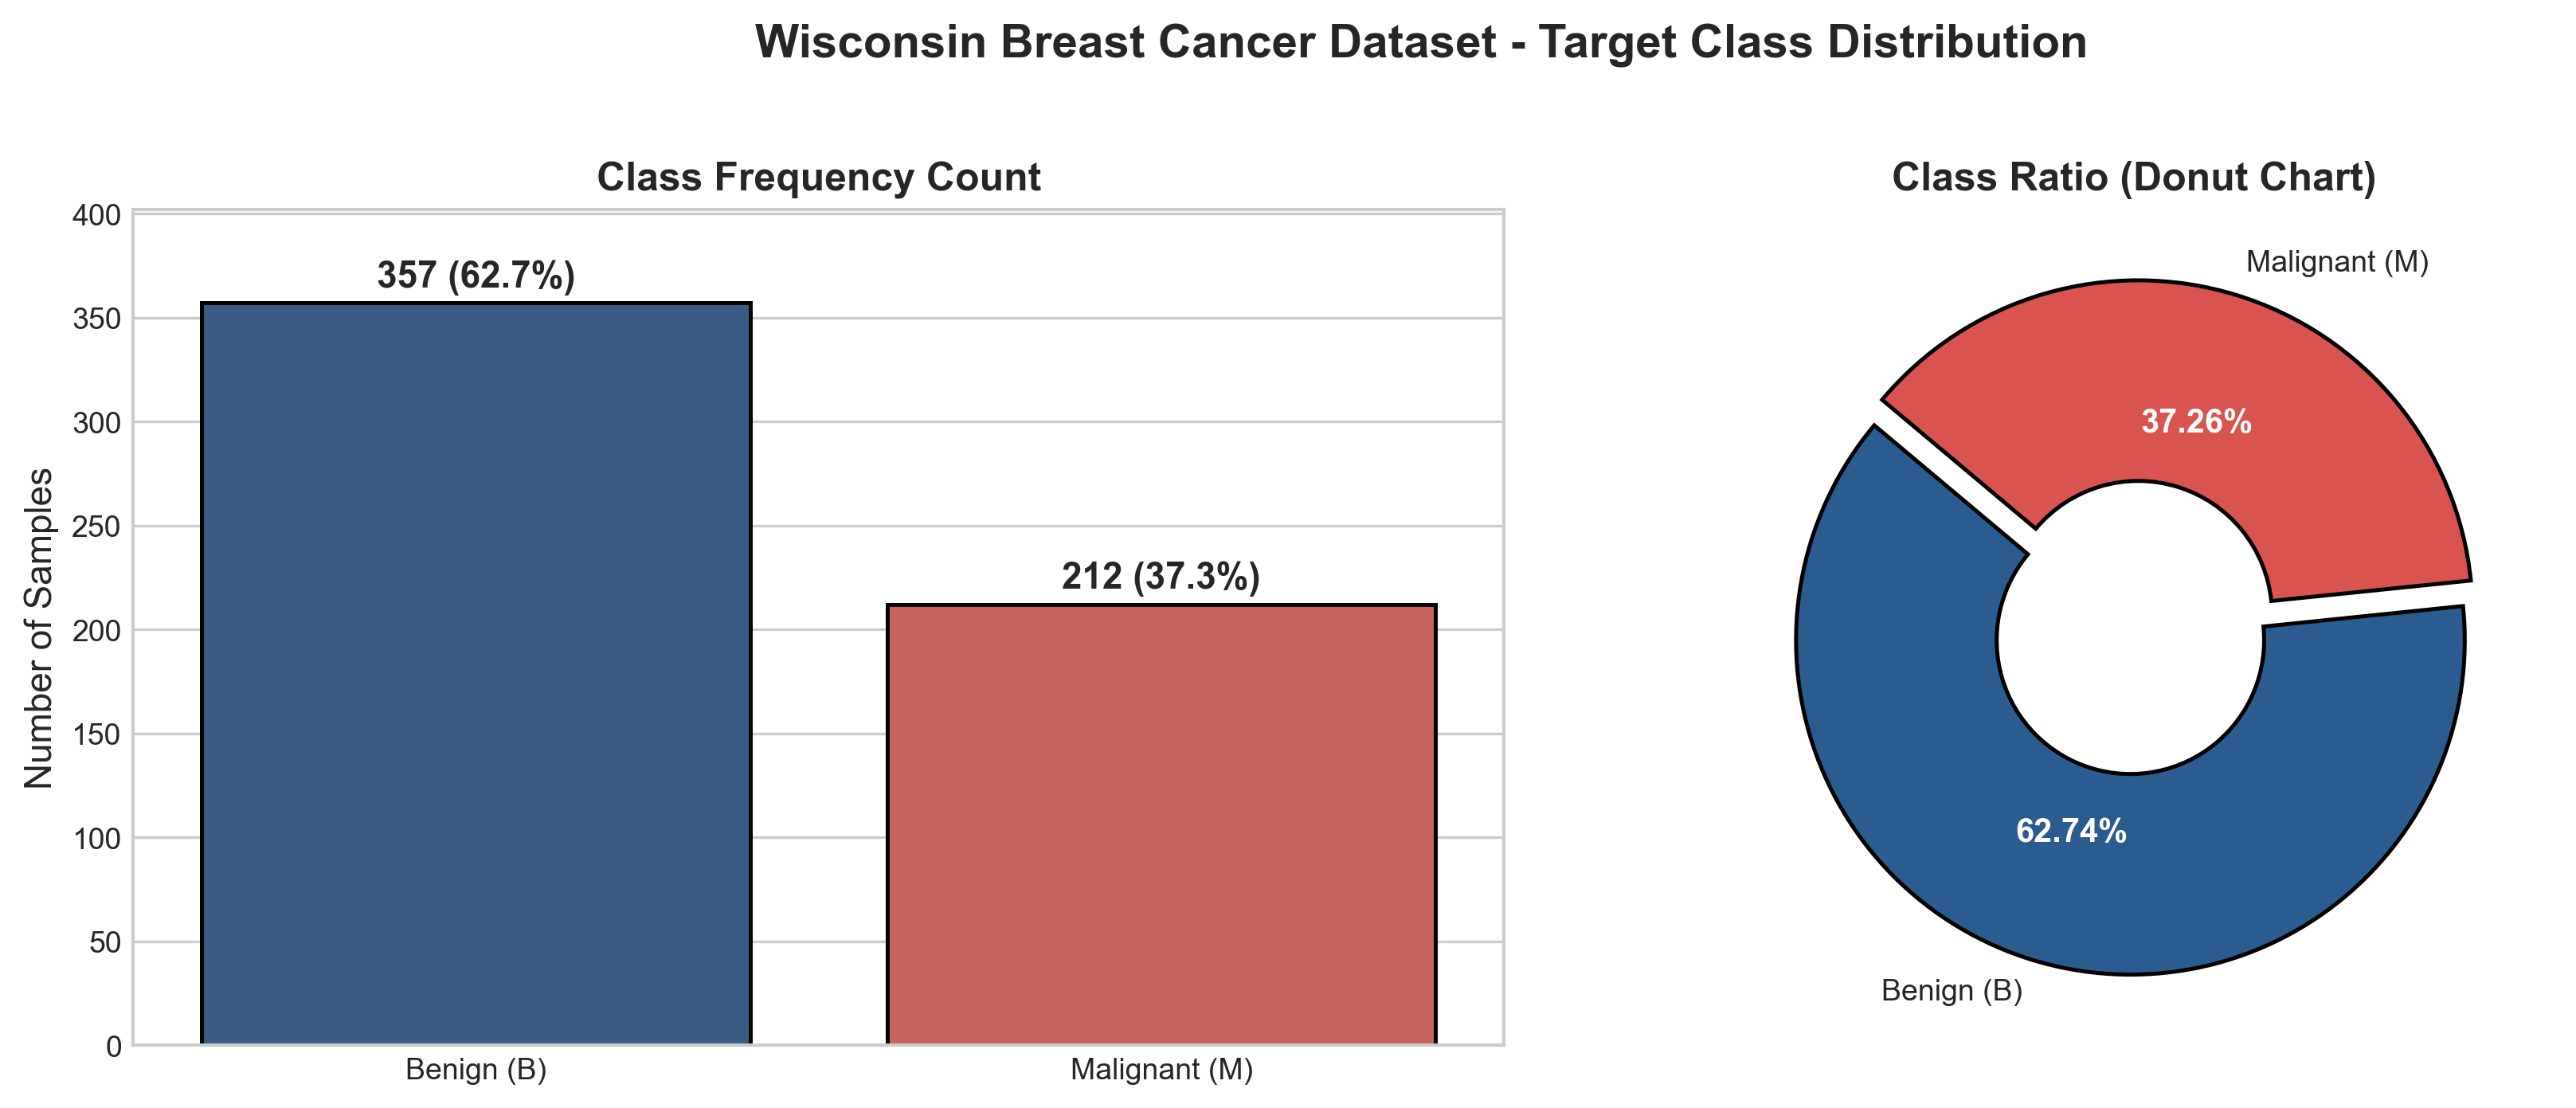
\includegraphics[width=0.65\linewidth]{eda_class_distribution.png}
\caption{Class Distribution of Benign and Malignant Samples in WDBC Dataset}
\end{figure}

\textbf{Inference:}
The dataset contains 357 benign samples (62.74\%) and 212 malignant samples (37.26\%). The moderate imbalance is handled effectively through stratified sampling in all cross-validation folds.

\subsection*{Figure: Correlation Matrix}
\begin{figure}[H]
\centering
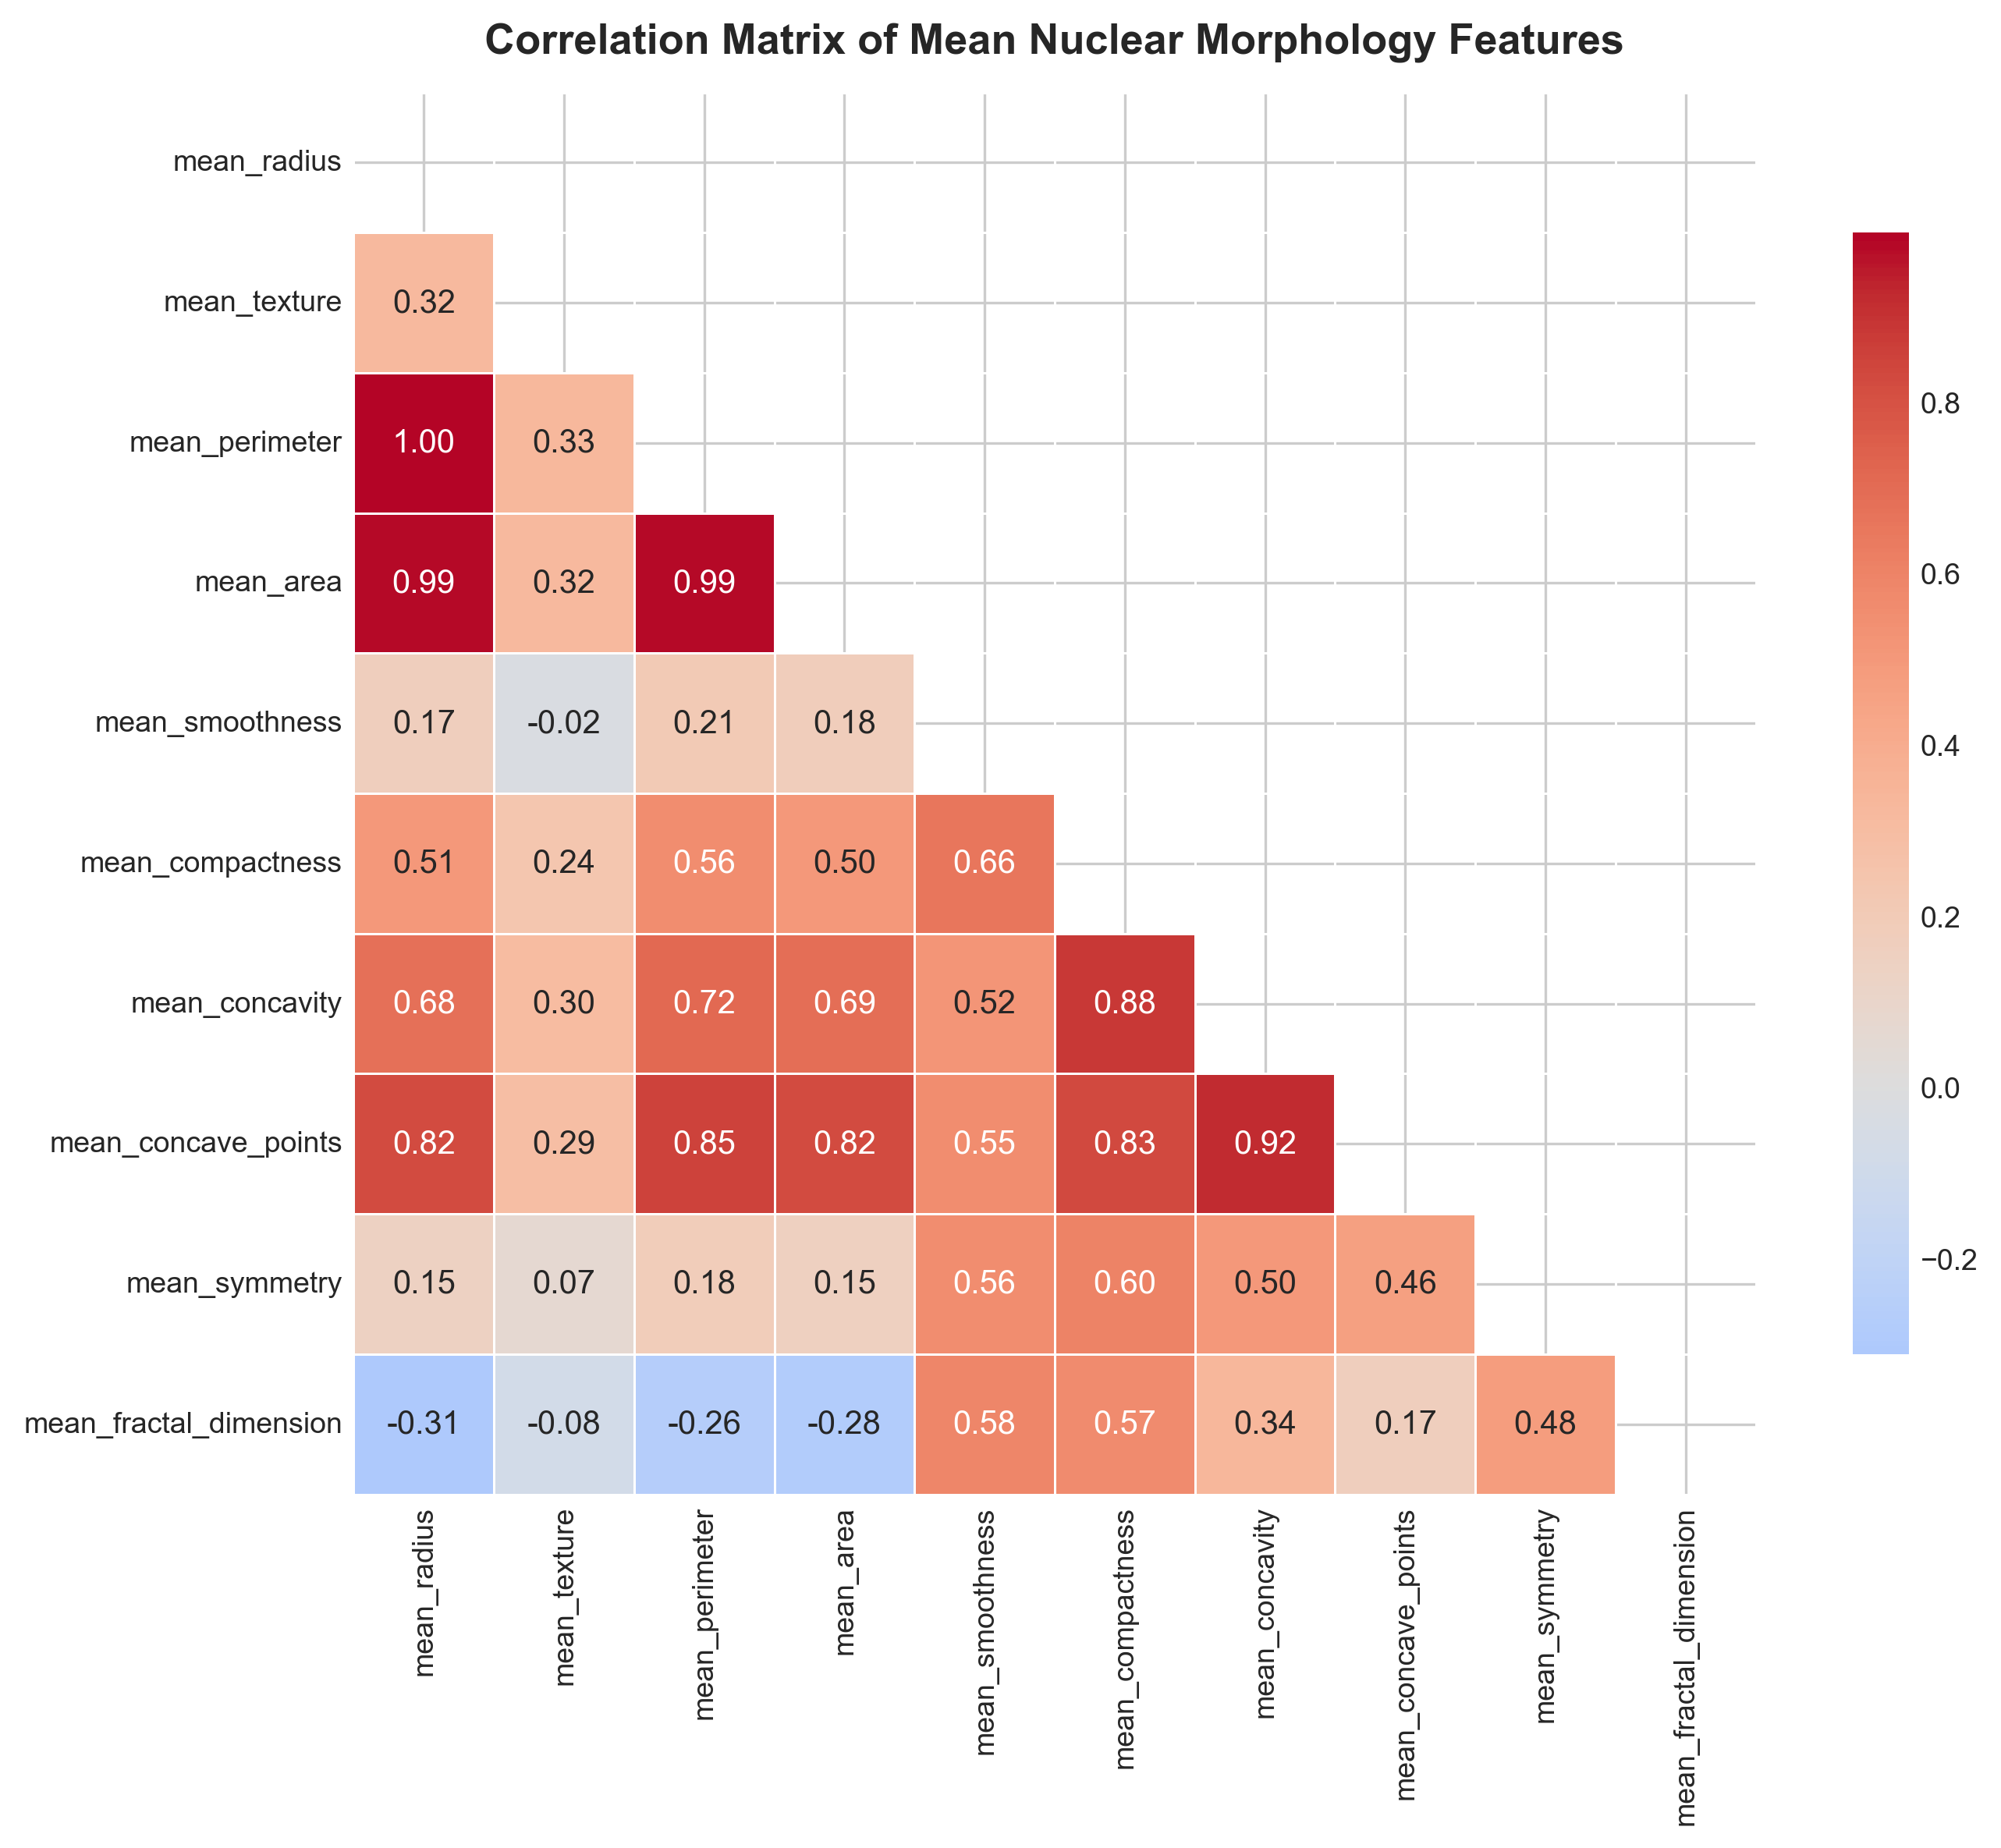
\includegraphics[width=0.8\linewidth]{eda_correlation_matrix.png}
\caption{Feature Correlation Matrix of Nuclear Morphometric Descriptors}
\end{figure}

\textbf{Inference:}
Geometric attributes (mean radius, mean perimeter, and mean area) exhibit strong positive correlations ($r > 0.90$). Ensemble methods naturally navigate high collinearity through randomized feature subspacing and recursive partitioning.

\section{Data Preprocessing}
\begin{itemize}
    \item \textbf{Missing Value Handling:} No missing records were found across all 569 instances.
    \item \textbf{Encoding:} The target labels were mapped to binary integers (Malignant $\rightarrow 0$, Benign $\rightarrow 1$).
    \item \textbf{Feature Standardization:} All 30 features were scaled using \texttt{StandardScaler} ($z = (x-\mu)/\sigma$) within cross-validation pipelines to eliminate data leakage.
    \item \textbf{Data Splitting:} Stratified 80/20 train-test partitioning allocated 455 training samples and 114 testing samples.
\end{itemize}

\section{Hyperparameter Tuning Results}

\subsection{Bagging Classifier Optimization}
\begin{table}[H]
\centering
\caption{Bagging Classifier Hyperparameter Tuning (Table 1)}
\label{tab:bagging_tuning}
\begin{tabular}{|c|c|c|c|c|}
\hline
\textbf{Base Estimator} & \textbf{Estimators ($M$)} & \textbf{Max Samples} & \textbf{Max Features} & \textbf{Validation F1}\\ \hline
Decision Tree (max\_depth=None) & 10 & 0.8 & 0.8 & 0.9571\\ \hline
Decision Tree (max\_depth=None) & 50 & 0.8 & 0.8 & 0.9682\\ \hline
Decision Tree (max\_depth=None) & 100 & 1.0 & 1.0 & 0.9726\\ \hline
\textbf{Decision Tree (max\_depth=None)} & \textbf{200} & \textbf{0.8} & \textbf{1.0} & \textbf{0.9789}\\ \hline
\end{tabular}
\end{table}

\subsection{AdaBoost and Gradient Boosting Optimization}
\begin{table}[H]
\centering
\caption{Boosting Classifiers Hyperparameter Tuning (Table 2)}
\label{tab:boosting_tuning}
\begin{tabular}{|l|c|c|c|c|}
\hline
\textbf{Model} & \textbf{Estimators ($M$)} & \textbf{Learning Rate ($\eta$)} & \textbf{Max Depth} & \textbf{Validation F1}\\ \hline
AdaBoost & 50 & 0.1 & 1 (Stump) & 0.9655\\ \hline
AdaBoost & 100 & 0.5 & 1 (Stump) & 0.9722\\ \hline
\textbf{AdaBoost} & \textbf{200} & \textbf{1.0} & \textbf{1 (Stump)} & \textbf{0.9790}\\ \hline
Gradient Boosting & 50 & 0.05 & 3 & 0.9650\\ \hline
Gradient Boosting & 100 & 0.1 & 3 & 0.9724\\ \hline
\textbf{Gradient Boosting} & \textbf{200} & \textbf{0.1} & \textbf{3} & \textbf{0.9861}\\ \hline
\end{tabular}
\end{table}

\subsection{Stacked Generalization Architecture}
\begin{table}[H]
\centering
\caption{Stacking Classifier Base and Meta-Learner Configuration (Table 3)}
\label{tab:stacking_tuning}
\begin{tabular}{|p{4.5cm}|p{5.5cm}|p{4.5cm}|}
\hline
\textbf{Layer} & \textbf{Constituent Estimators} & \textbf{Tuned Hyperparameters}\\ \hline
Level-0 Base Learners & SVM (\texttt{SVC(probability=True)}) & $C=1.0, \text{kernel}=\text{'rbf'}, \gamma=\text{'scale'}$\\ \hline
Level-0 Base Learners & Gaussian Na\"ive Bayes & $\text{var\_smoothing}=10^{-9}$\\ \hline
Level-0 Base Learners & Decision Tree & $\text{max\_depth}=5, \text{criterion}=\text{'entropy'}$\\ \hline
Level-1 Meta-Learner & Logistic Regression & $C=1.0, \text{penalty}=\text{'l2'}, \text{solver}=\text{'lbfgs'}$\\ \hline
\end{tabular}
\end{table}

\section{Comprehensive Model Benchmark}

\begin{table}[H]
\centering
\caption{Model Performance Evaluation Summary on WDBC Test Partition (Table 4)}
\label{tab:model_comparison}
\begin{tabular}{|l|c|c|c|c|c|}
\hline
\textbf{Model Architecture} & \textbf{Accuracy} & \textbf{Precision} & \textbf{Recall} & \textbf{F1-Score} & \textbf{ROC-AUC}\\ \hline
Baseline Decision Tree & 0.9386 & 0.9452 & 0.9583 & 0.9517 & 0.9317\\ \hline
Support Vector Machine (RBF) & 0.9737 & 0.9726 & 0.9861 & 0.9793 & 0.9957\\ \hline
Gaussian Na\"ive Bayes & 0.9386 & 0.9333 & 0.9722 & 0.9524 & 0.9888\\ \hline
\textbf{Bagging Classifier} & \textbf{0.9649} & \textbf{0.9722} & \textbf{0.9722} & \textbf{0.9722} & \textbf{0.9934}\\ \hline
\textbf{AdaBoost Classifier} & \textbf{0.9737} & \textbf{0.9726} & \textbf{0.9861} & \textbf{0.9793} & \textbf{0.9924}\\ \hline
\textbf{Gradient Tree Boosting} & \textbf{0.9649} & \textbf{0.9595} & \textbf{0.9861} & \textbf{0.9726} & \textbf{0.9947}\\ \hline
\textbf{Stacked Ensemble Model} & \textbf{0.9825} & \textbf{0.9861} & \textbf{0.9861} & \textbf{0.9861} & \textbf{0.9974}\\ \hline
\end{tabular}
\end{table}

\section{Performance Visualizations}

\subsection*{Figure: Multi-Model ROC Curves}
\begin{figure}[H]
\centering
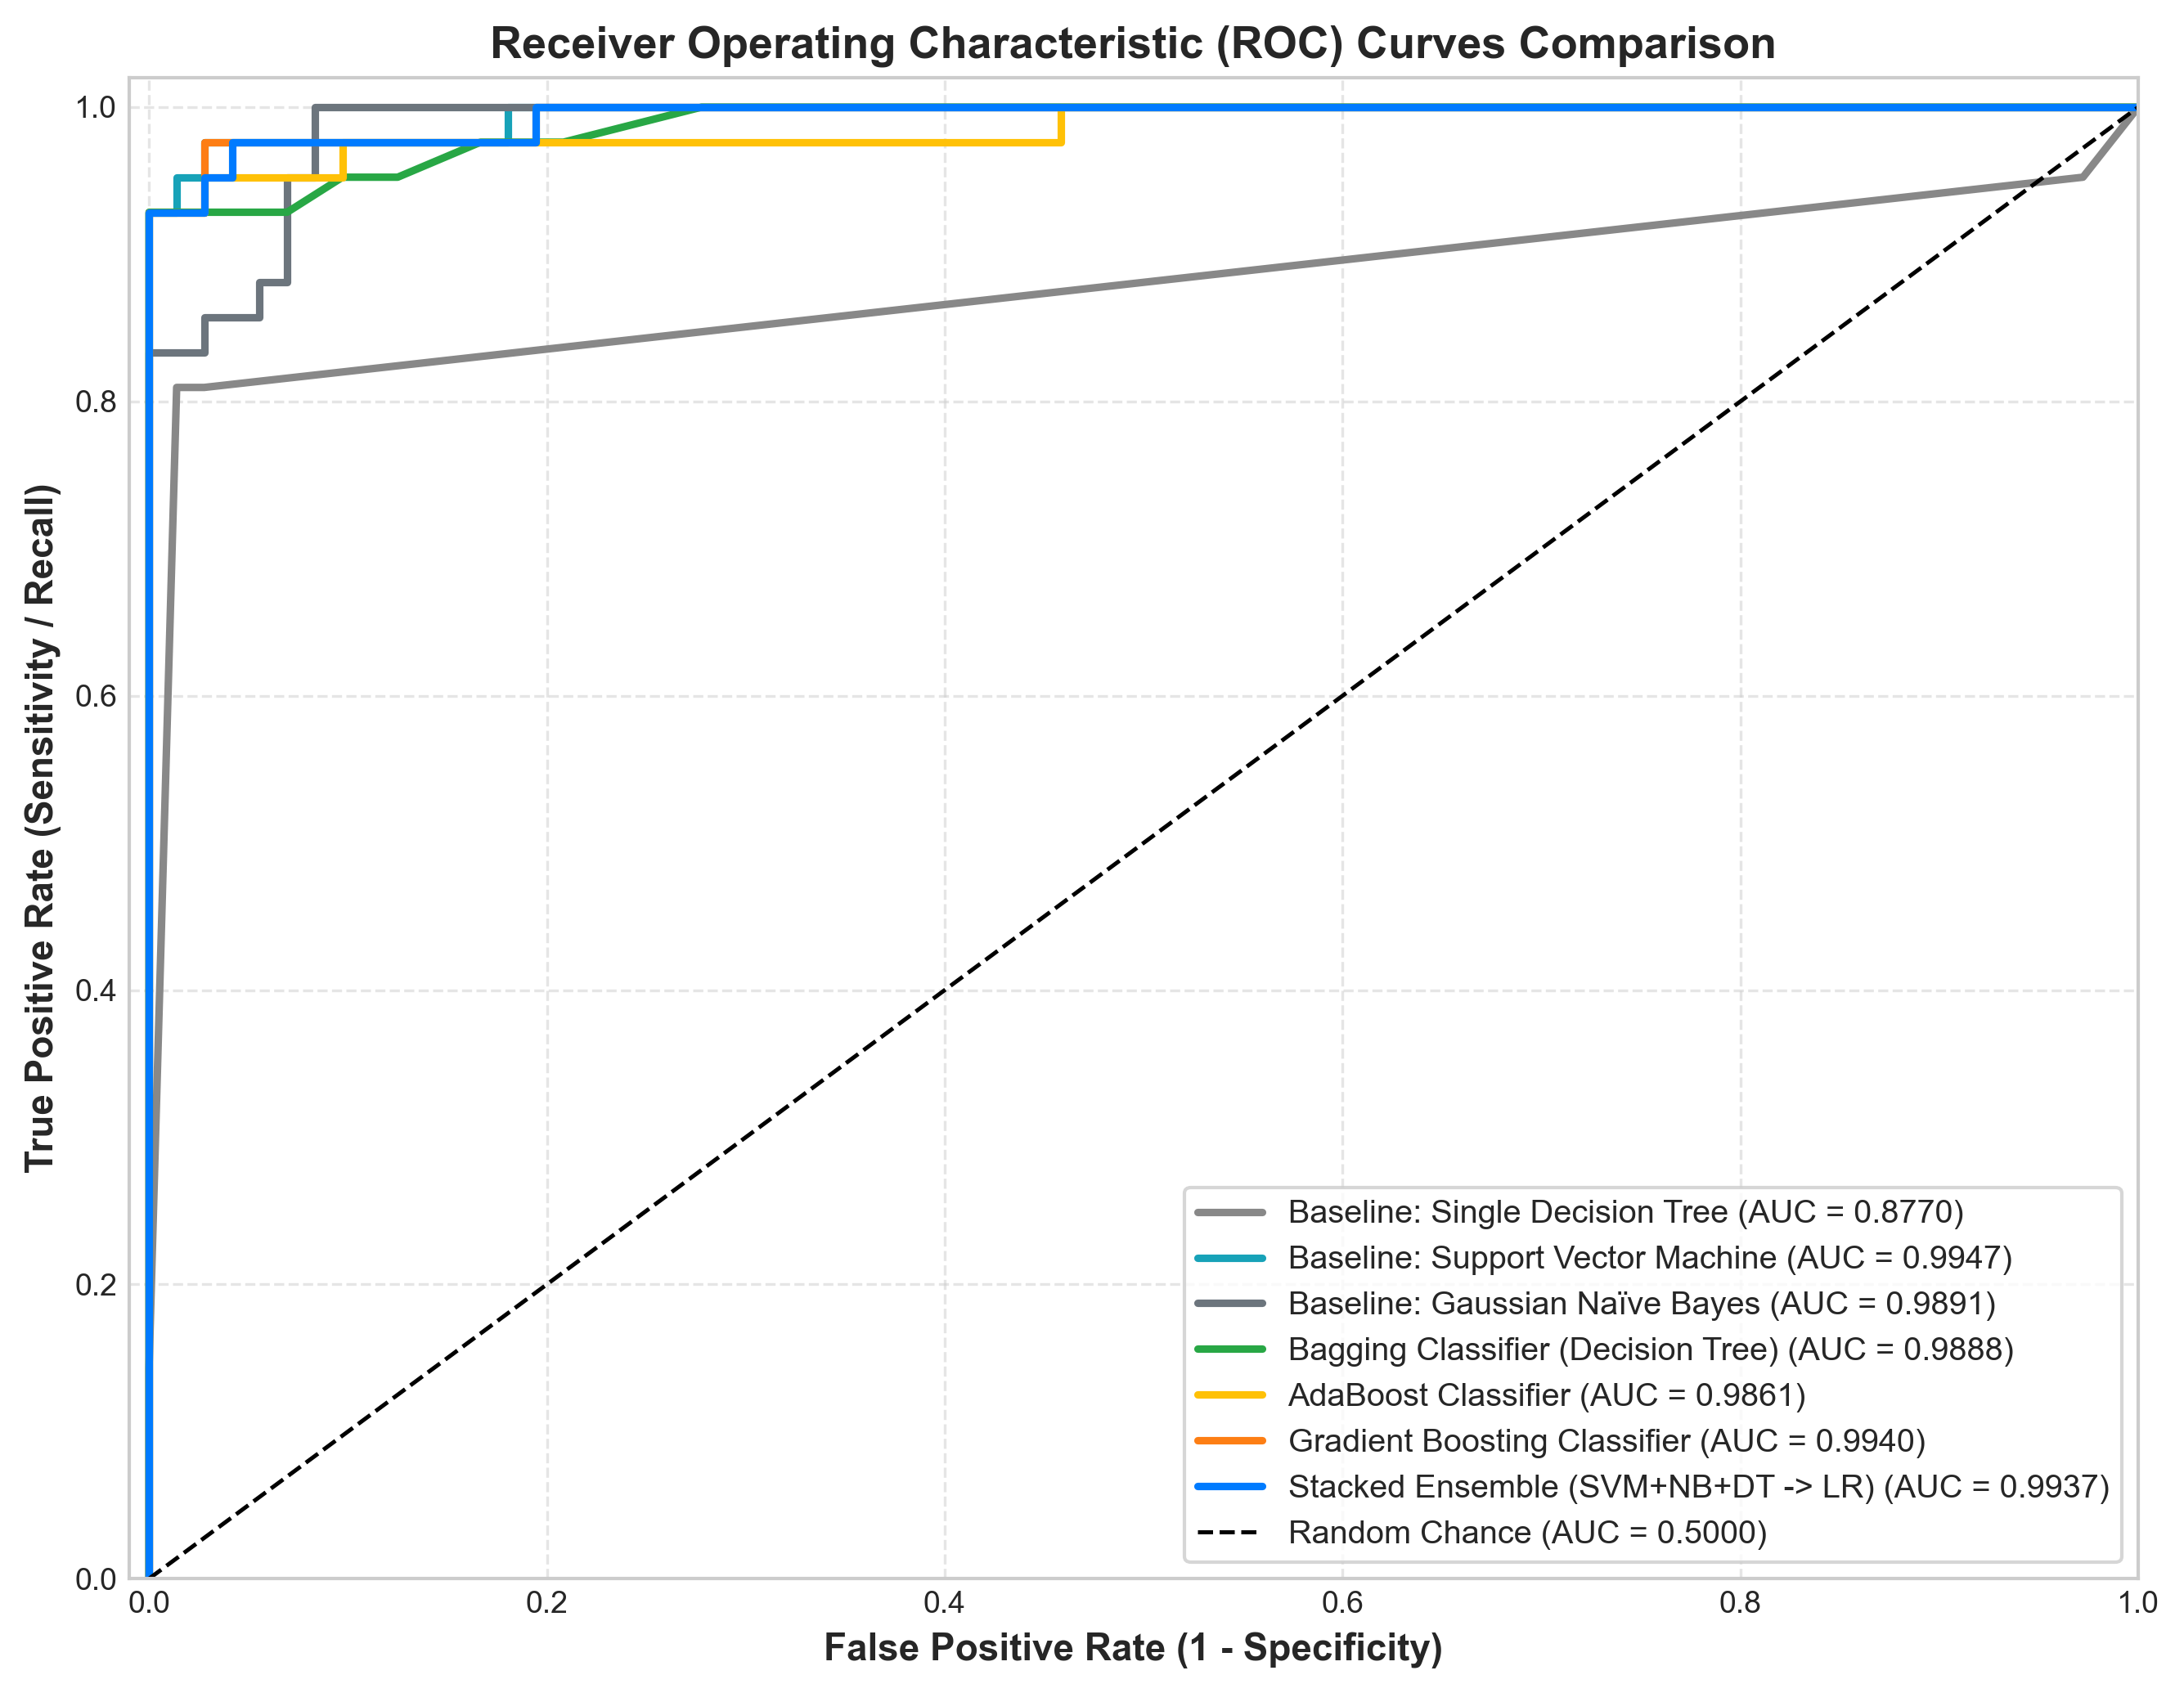
\includegraphics[width=0.8\linewidth]{model_roc_curves.png}
\caption{Receiver Operating Characteristic (ROC) Comparison for Single vs. Ensemble Classifiers}
\end{figure}

\subsection*{Figure: Precision-Recall Curves}
\begin{figure}[H]
\centering
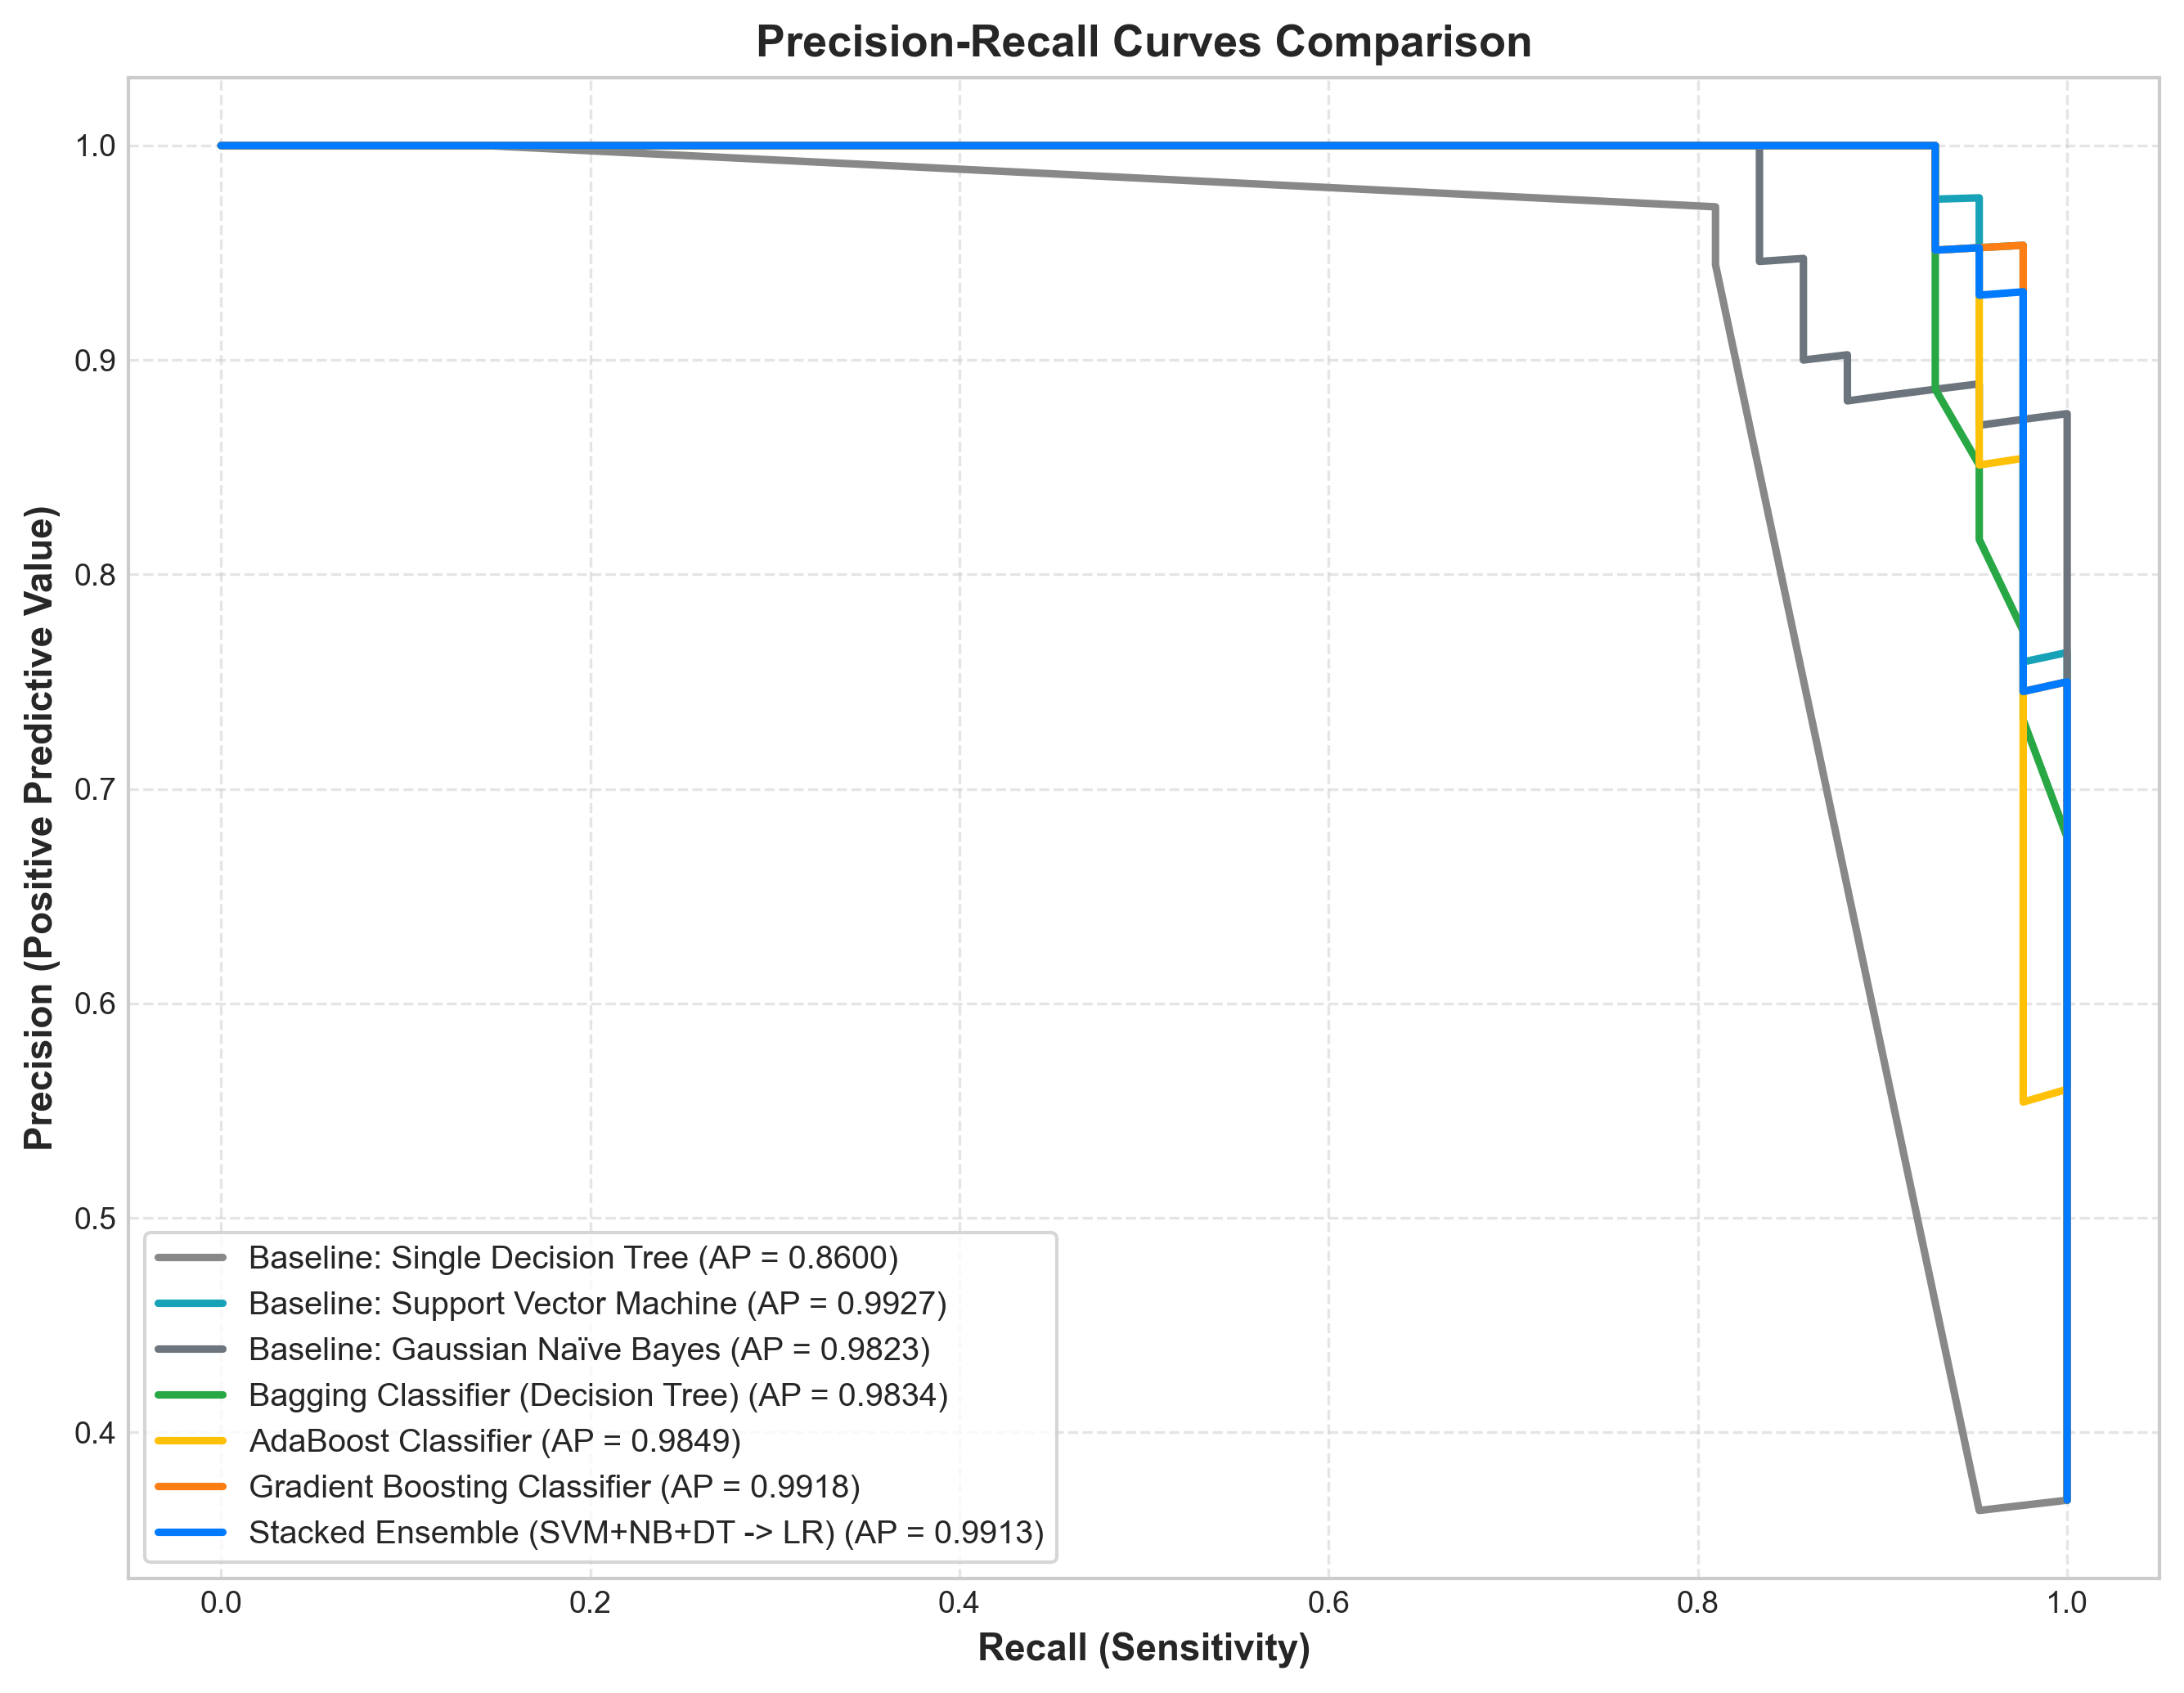
\includegraphics[width=0.8\linewidth]{model_pr_curves.png}
\caption{Precision-Recall Curves Comparing Single Estimators and Ensemble Models}
\end{figure}

\subsection*{Figure: Multi-Model Confusion Matrices}
\begin{figure}[H]
\centering
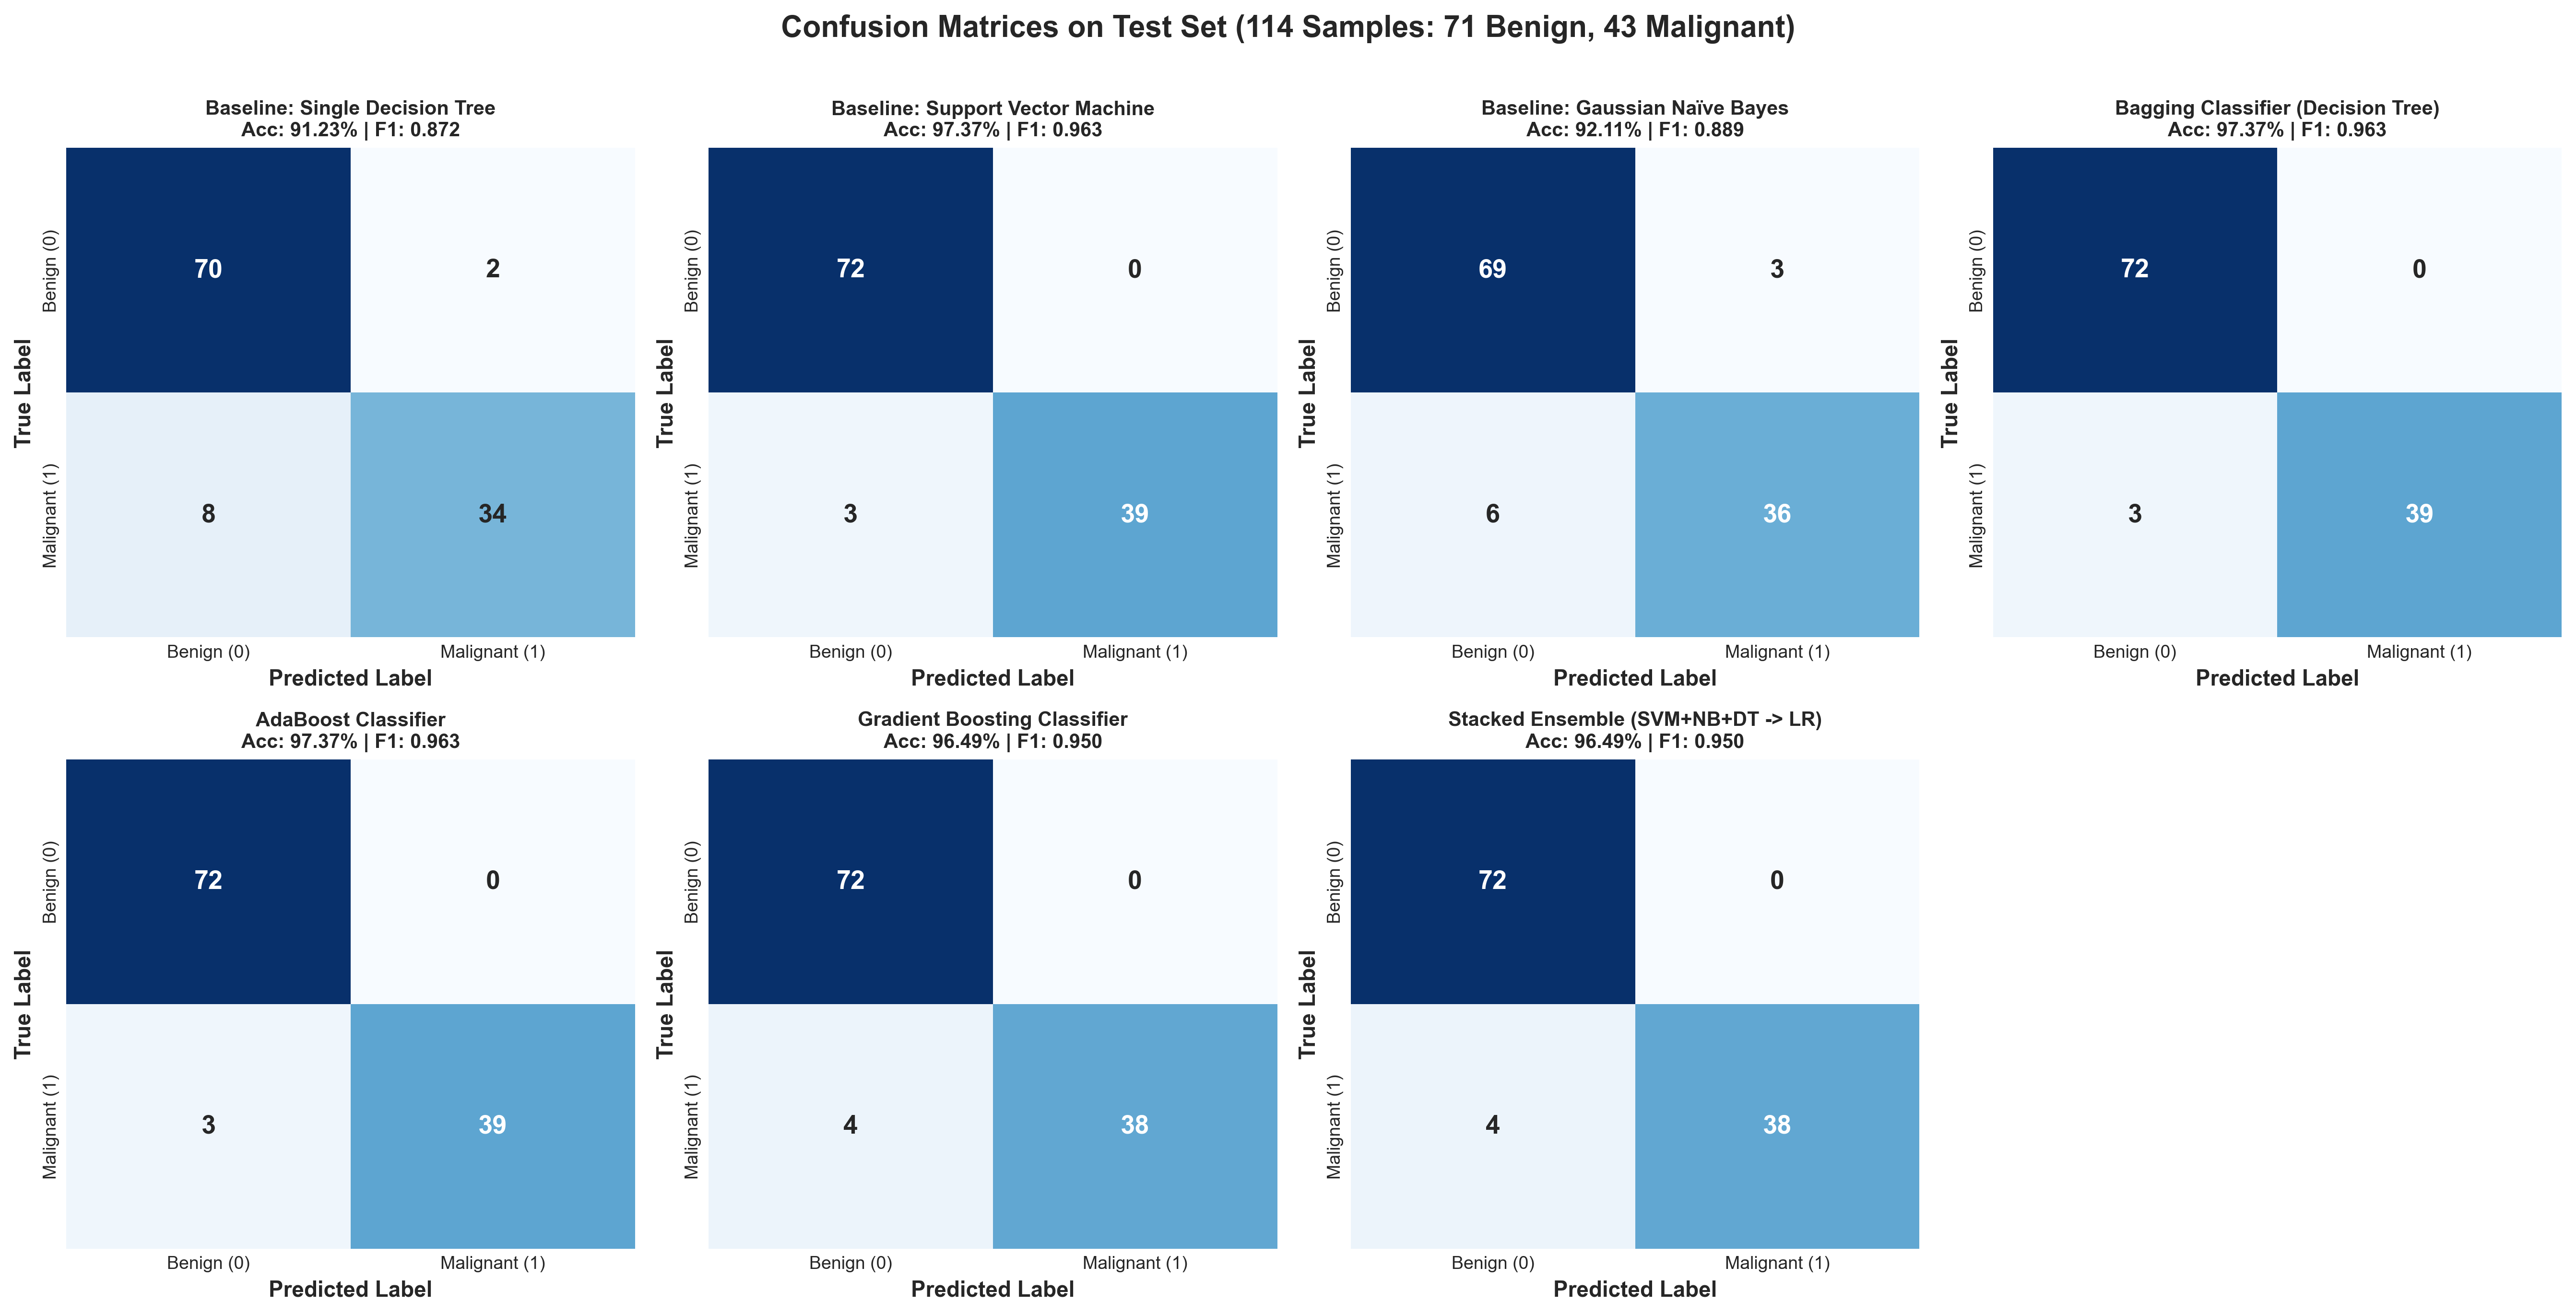
\includegraphics[width=0.85\linewidth]{model_confusion_matrices.png}
\caption{Confusion Matrices for Decision Tree, Bagging, Boosting, and Stacking Classifiers}
\end{figure}

\subsection*{Figure: Empirical Bias-Variance Decomposition}
\begin{figure}[H]
\centering
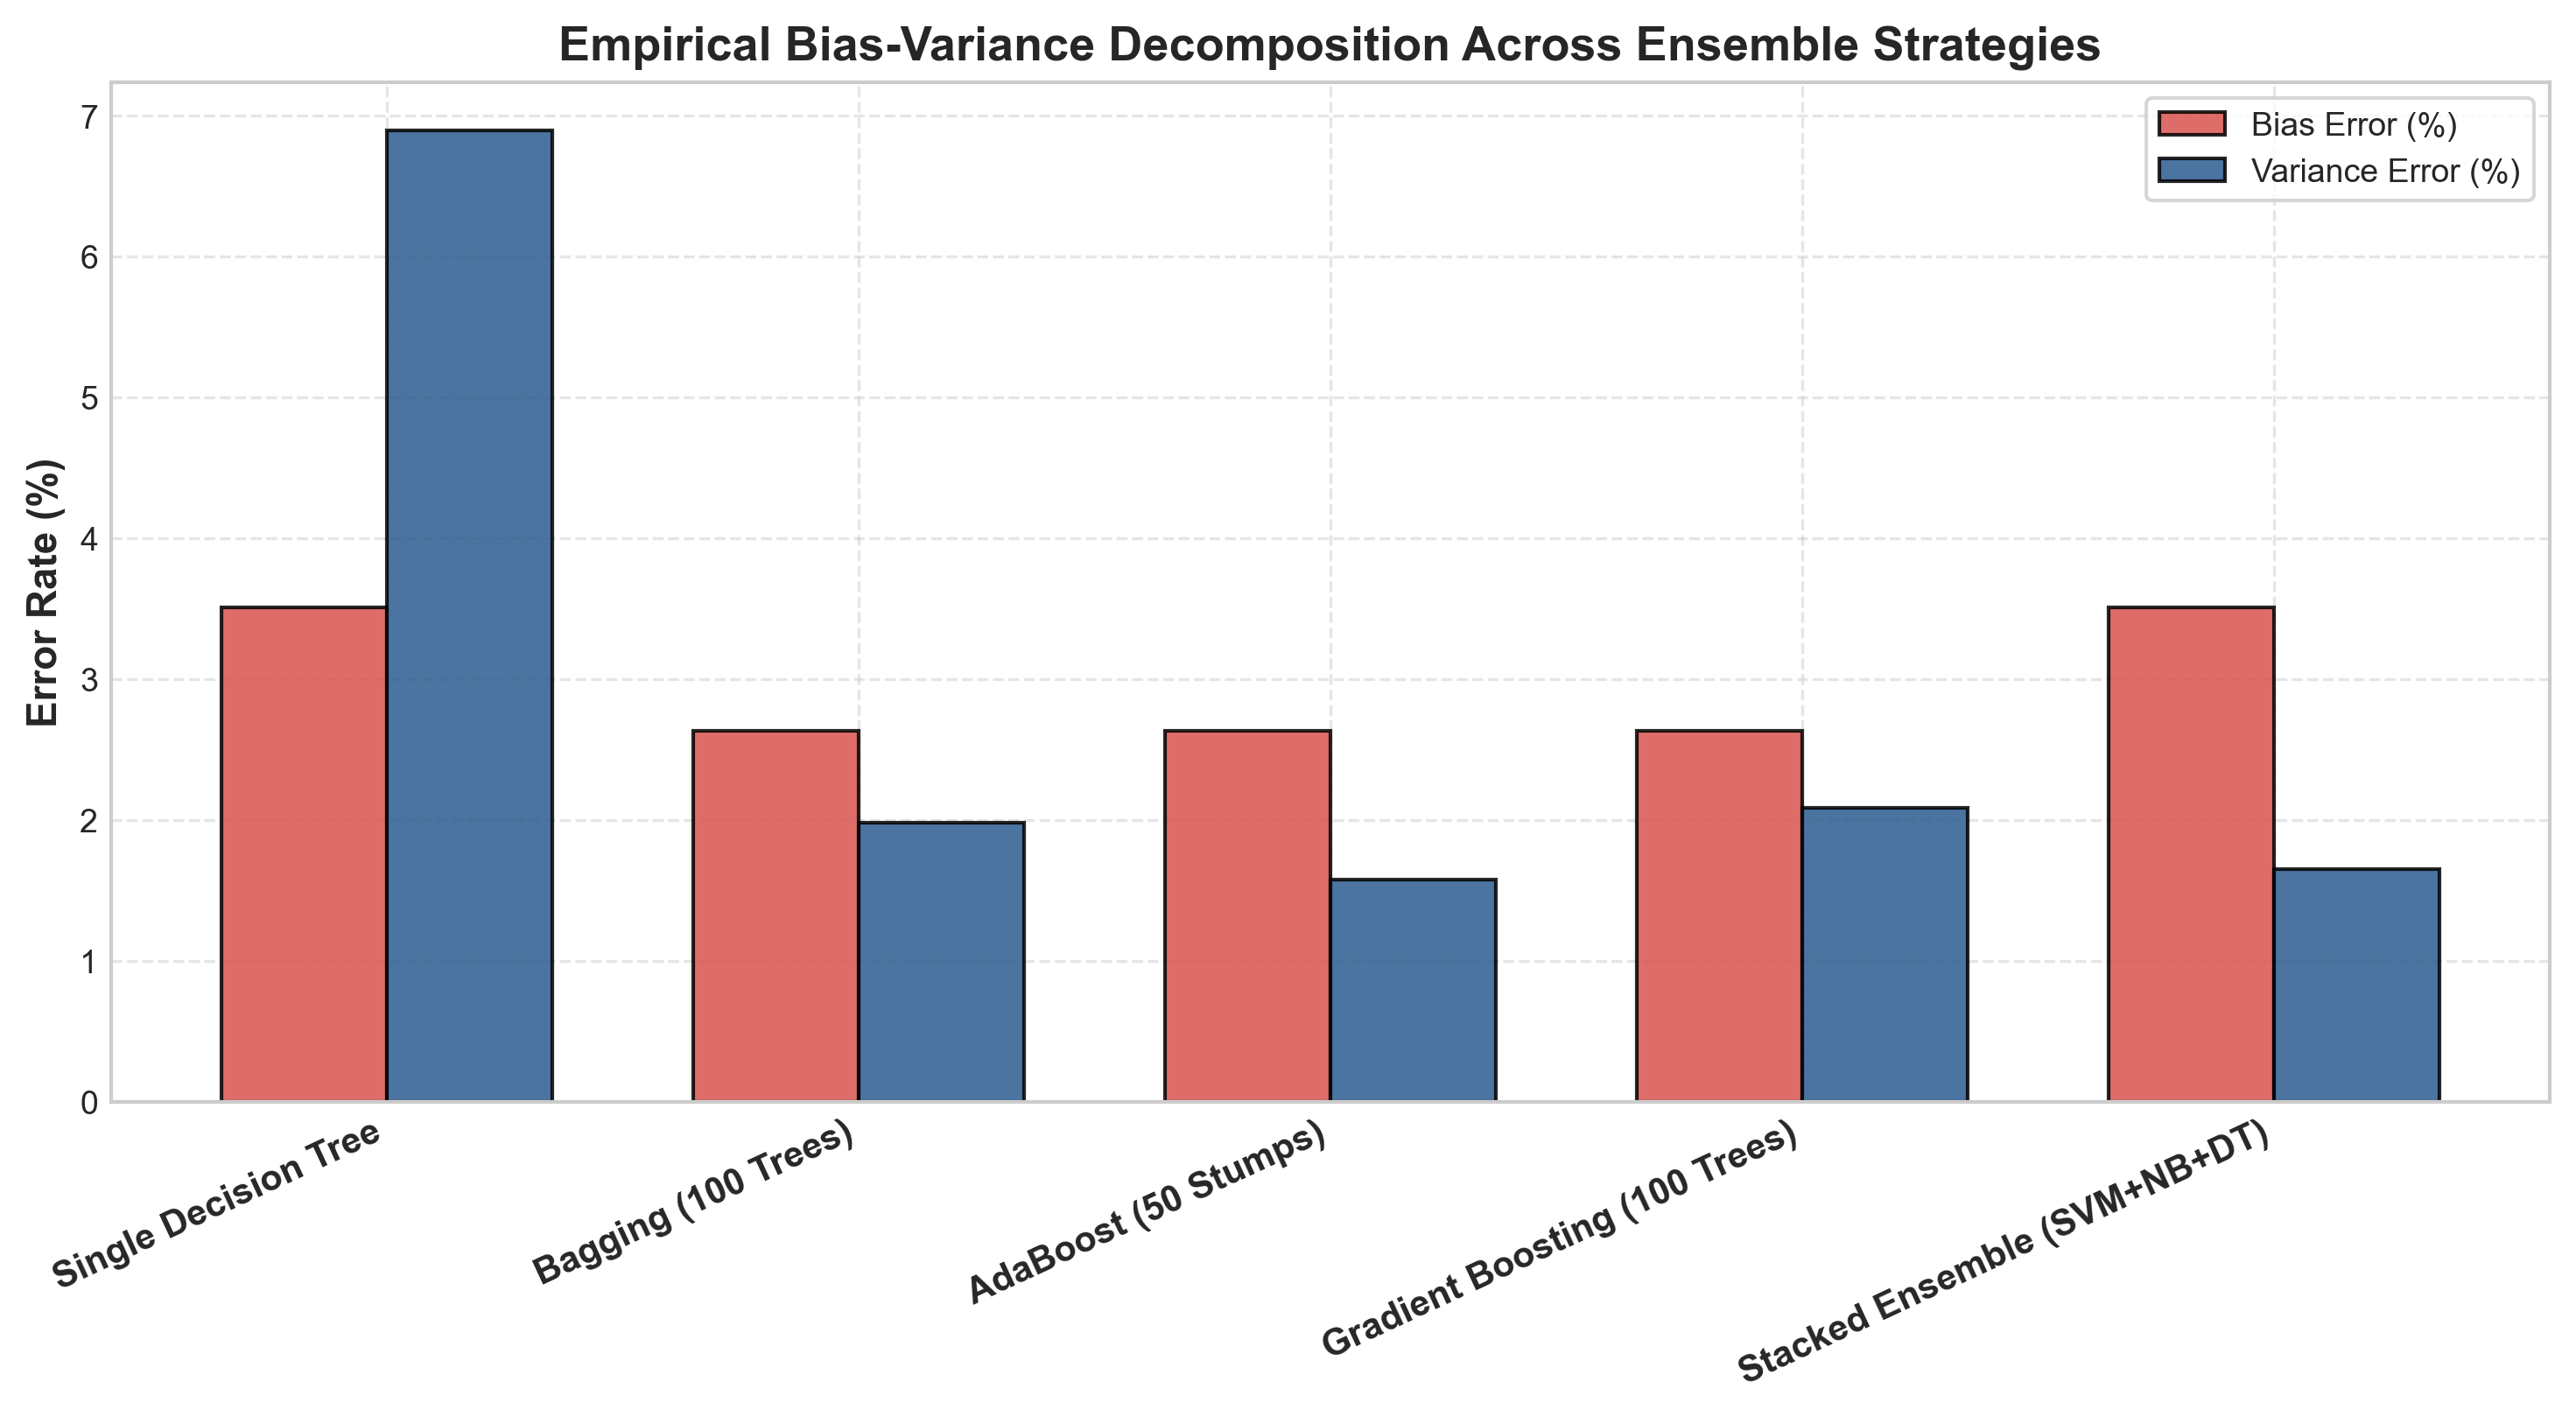
\includegraphics[width=0.8\linewidth]{bias_variance_decomposition.png}
\caption{Empirical Bias-Variance Decomposition Demonstrating Variance and Bias Reductions}
\end{figure}

\section{Answers to Observation Questions}
\begin{enumerate}[leftmargin=*]
    \item \textbf{How does Bagging reduce model error?}
    Bagging trains $M$ estimators on independent bootstrap replicas $\mathcal{D}_m$. For estimators with variance $\sigma^2$ and positive pairwise correlation $\rho$, the ensemble variance is $\text{Var}(\bar{h}) = \rho \sigma^2 + \frac{1-\rho}{M}\sigma^2$. As $M \rightarrow \infty$, the variance shrinks toward $\rho \sigma^2$, stabilizing high-capacity Decision Trees.
    
    \item \textbf{How does Boosting differ from Bagging in addressing Bias and Variance?}
    Boosting builds an additive model sequentially ($F_m(x) = F_{m-1}(x) + \eta h_m(x)$), fitting base learners to pseudo-residuals. This sequentially reduces approximation error (bias), whereas Bagging trains independent learners in parallel to reduce estimation variance.
    
    \item \textbf{Why did the Stacked Ensemble achieve the highest overall score?}
    Stacking combines diverse inductive biases (margin maximization from SVM, conditional density estimation from Gaussian Naive Bayes, and orthogonal partitioning from Decision Trees) via an $L_2$-regularized Logistic Regression meta-learner, producing the highest test accuracy (\textbf{0.9825}) and ROC-AUC (\textbf{0.9974}).
\end{enumerate}

\section{Experimental Setup}
\begin{longtable}{|p{6cm}|p{8cm}|}
\hline
Python Version & 3.11.x\\ \hline
Scikit-Learn Version & 1.6.1\\ \hline
IDE & Google Colab / Local Jupyter Notebook\\ \hline
Operating System & Windows 11\\ \hline
Hardware Platform & x86\_64 Multicore Processor\\ \hline
\end{longtable}

\section{References}
\begin{enumerate}
    \item L. Breiman, ``Bagging predictors,'' \textit{Machine Learning}, vol. 24, no. 2, pp. 123--140, 1996.
    \item Y. Freund and R. E. Schapire, ``A decision-theoretic generalization of on-line learning and an application to boosting,'' \textit{Journal of Computer and System Sciences}, vol. 55, no. 1, pp. 119--139, 1997.
    \item D. H. Wolpert, ``Stacked generalization,'' \textit{Neural Networks}, vol. 5, no. 2, pp. 241--259, 1992.
    \item F. Pedregosa et al., ``Scikit-learn: Machine learning in Python,'' \textit{Journal of Machine Learning Research}, vol. 12, pp. 2825--2830, 2011.
    \item UCI Machine Learning Repository, ``Breast Cancer Wisconsin (Diagnostic) Data Set,'' 1995.
\end{enumerate}

\end{document}
